\documentclass{beamer}

\usepackage[utf8]{inputenc} 
\usepackage[T1]{fontenc}
\usepackage{lmodern}
\usepackage{graphicx}
\usepackage[french]{babel}

%====================================
%===load master thesis config file===
%====================================


\beamertemplatenavigationsymbolsempty
%\setbeamerfont{page number in head/foot}{size=\large}
\setbeamertemplate{footline}[frame number]

\usetheme{Darmstadt}
%\usetheme{Goettingen}
\useinnertheme{circles}

\mode<presentation>

\useoutertheme[footline=authortitle]{miniframes}
%\useinnertheme{circles}
%\usecolortheme{whale}
\usecolortheme{beaver}

\usepackage{listings}

%\usepackage{beamerthemeAmsterdam}
%\setbeamertemplate{navigation symbols}{}
\providecommand{\tightlist}{%
  \setlength{\itemsep}{0pt}\setlength{\parskip}{0pt}}
  
%=============
%=== title ===
%=============
\title{Introduction to C programming}
\subtitle{Basic examples for the chipkit mx4 board}
\author{Dimitri de Smet}
\institute{UCL}
\date{\today}

%==============
%===document===
%==============

%==============
%===document===
%==============

\begin{document}

%==================
%=== title page ===
%==================

\begin{frame}
\titlepage
\end{frame}

%\begin{frame}
%\frametitle{Outline}
%\tableofcontents
%\end{frame}


%=================
%=== main part ===
%=================

\begin{frame}{Reminders}

\begin{itemize}
\tightlist
\item
  Computer architecture
\item
  Code/compile/program
\item
  Your computer board
\end{itemize}

\end{frame}

\begin{frame}{Today's plan}

\begin{itemize}
\tightlist
\item
  C language examples
\item
  Tools installation and exercices
\end{itemize}

\end{frame}

\begin{frame}{Softwares}

\begin{itemize}
\tightlist
\item
  \href{http://www.microchip.com/mplab/mplab-x-ide?tab=t2}{MPLAB X IDE}
\item
  \href{http://www.microchip.com/mplab/compilers}{XC32 compiler}
\end{itemize}

Download and intall the last version under the ``Download Archive'' tab.

\end{frame}

\begin{frame}{Example 0}

\lstinputlisting[firstline=12,lastline=13,language=c]{../../code/mrk-board/intro_examples/sources/main.c}

\lstinputlisting[firstline=17,lastline=19,language=c]{../../code/mrk-board/intro_examples/sources/main.c}

\lstinputlisting[firstline=280,lastline=284,language=c]{../../code/mrk-board/intro_examples/sources/main.c}

\end{frame}

\begin{frame}{Lessons}

\begin{enumerate}
\def\labelenumi{\arabic{enumi}.}
\tightlist
\item
  Comments : \emph{//}
\item
  Main function : \emph{void main(void)}
\item
  An instruction line ends with `;'
\item
  Functions and levels of abstraction

  \begin{itemize}
  \tightlist
  \item
    Hierarchy
  \end{itemize}
\end{enumerate}

\end{frame}

\begin{frame}{Example 1}

\lstinputlisting[firstline=35,lastline=39,language=c]{../../code/mrk-board/intro_examples/sources/main.c}

\end{frame}

\begin{frame}{Lessons}

\begin{enumerate}
\def\labelenumi{\arabic{enumi}.}
\tightlist
\item
  Digital outputs
\item
  Arguments of a function between `( )'
\item
  Hexa notation
\item
  Levels of abstraction

  \begin{itemize}
  \tightlist
  \item
    Modularity
  \end{itemize}
\item
  Function initIO()
\end{enumerate}

\end{frame}

\begin{frame}{Example 2}

\lstinputlisting[firstline=41,lastline=48,language=c]{../../code/mrk-board/intro_examples/sources/main.c}

\end{frame}

\begin{frame}{Lessons}

\begin{enumerate}
\def\labelenumi{\arabic{enumi}.}
\tightlist
\item
  Digital intputs
\item
  \emph{if(\ldots{}) \ldots{} else}
\item
  Binary notation
\item
  The \emph{main} function is executed once
\end{enumerate}

\end{frame}

\begin{frame}{Example 3}

\lstinputlisting[firstline=50,lastline=59,language=c]{../../code/mrk-board/intro_examples/sources/main.c}

\end{frame}

\begin{frame}{Lessons}

\begin{enumerate}
\def\labelenumi{\arabic{enumi}.}
\tightlist
\item
  while(1) = infinite loop
\item
  \emph{setLeds( getButton2() );}
\end{enumerate}

\end{frame}

\begin{frame}{Example 4}

\lstinputlisting[firstline=61,lastline=73,language=c]{../../code/mrk-board/intro_examples/sources/main.c}

\end{frame}

\begin{frame}{Lessons}

\begin{enumerate}
\def\labelenumi{\arabic{enumi}.}
\tightlist
\item
  Variable declaration (here type \emph{char})
\item
  Logic operators
\end{enumerate}

\begin{center}
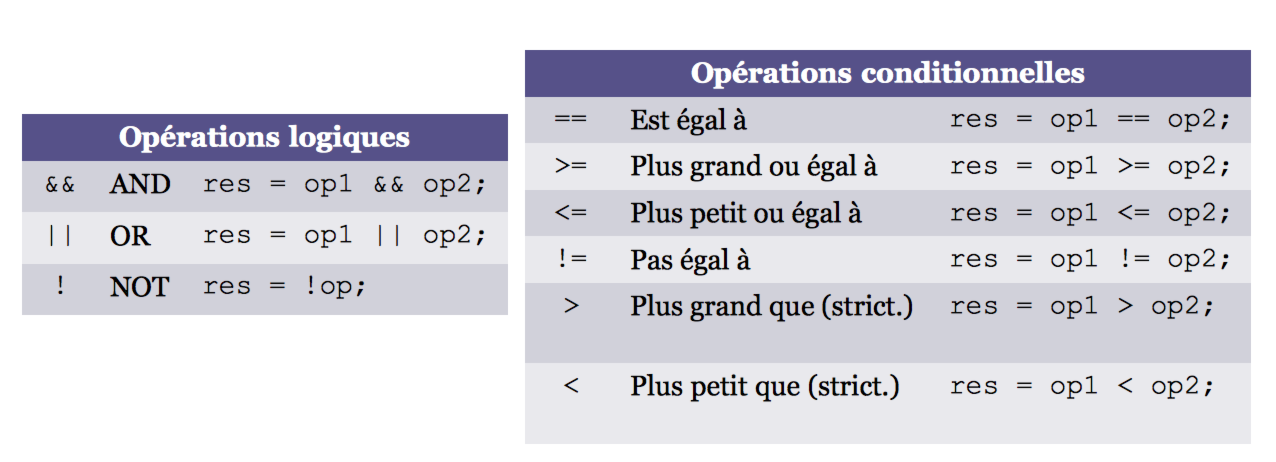
\includegraphics[width=1\textwidth]{images/logique.png}
\end{center}

\begin{itemize}
\tightlist
\item
  ? If( (x \textgreater{} 4) \&\& (x \textless{} 10) )
\end{itemize}

\end{frame}

\begin{frame}{Example 5}

\lstinputlisting[firstline=76,lastline=84,language=c]{../../code/mrk-board/intro_examples/sources/main.c}

\end{frame}

\begin{frame}{Lessons}

\begin{enumerate}
\def\labelenumi{\arabic{enumi}.}
\tightlist
\item
  Typical structure of our programs
\item
  CPU frequency : 10 MHz
\item
  Bitwise operators
\end{enumerate}

\begin{center}
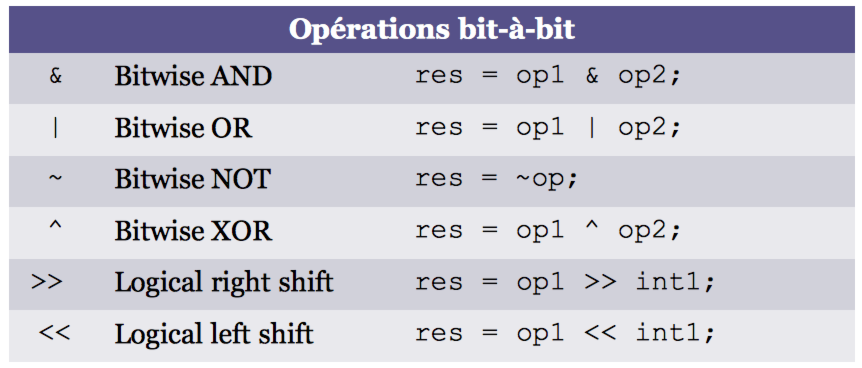
\includegraphics[width=.7\textwidth]{images/logique2.png}
\end{center}

\begin{itemize}
\tightlist
\item
  ??

  \begin{itemize}
  \tightlist
  \item
    leds = 0xaa \& 0xf0
  \item
    leds = 0xaa \&\& 0xf0
  \end{itemize}
\end{itemize}

\end{frame}

\begin{frame}{Example 6}

\lstinputlisting[firstline=86,lastline=99,language=c]{../../code/mrk-board/intro_examples/sources/main.c}

\end{frame}

\begin{frame}{Lessons}

\begin{enumerate}
\def\labelenumi{\arabic{enumi}.}
\tightlist
\item
  Execution time
\end{enumerate}

\end{frame}

\begin{frame}{Example 7 (1/2)}

\lstinputlisting[firstline=101,lastline=108,language=c]{../../code/mrk-board/intro_examples/sources/main.c}

\end{frame}

\begin{frame}{Example 7 (2/2)}

\lstinputlisting[firstline=29,lastline=33,language=c]{../../code/mrk-board/intro_examples/sources/main.c}

\end{frame}

\begin{frame}{Lessons}

\begin{enumerate}
\def\labelenumi{\arabic{enumi}.}
\tightlist
\item
  Modularity
\end{enumerate}

\end{frame}

\begin{frame}{Example 8}

\lstinputlisting[firstline=110,lastline=121,language=c]{../../code/mrk-board/intro_examples/sources/main.c}

\end{frame}

\begin{frame}{Lessons}

\begin{enumerate}
\def\labelenumi{\arabic{enumi}.}
\tightlist
\item
  New functions provided by \emph{delay.h}

  \begin{itemize}
  \tightlist
  \item
    \emph{initDelay()}
  \item
    \emph{DelayMs(int tms)}
  \item
    \emph{DelayUs(short tus)}
  \end{itemize}
\end{enumerate}

\end{frame}

\begin{frame}{Example 9}

\lstinputlisting[firstline=123,lastline=132,language=c]{../../code/mrk-board/intro_examples/sources/main.c}

\end{frame}

\begin{frame}{Lessons}

\begin{enumerate}
\def\labelenumi{\arabic{enumi}.}
\tightlist
\item
  Analog inputs
\item
  10-bits conversion
\item
  4-bits display
\end{enumerate}

\end{frame}

\begin{frame}{Example 10}

\lstinputlisting[firstline=135,lastline=145,language=c]{../../code/mrk-board/intro_examples/sources/main.c}

\end{frame}

\begin{frame}{Lessons}

\begin{enumerate}
\def\labelenumi{\arabic{enumi}.}
\tightlist
\item
  16 x 2 characters screen
\item
  Table of variable (here table of char)
\item
  functions provided by \emph{PmodCLP.h}

  \begin{itemize}
  \tightlist
  \item
    \emph{void initLCD();}
  \item
    \emph{void writeLine(char * string, char line);}
  \item
    \emph{void clearScreen();}
  \item
    \emph{void shiftScreen(unsigned char right);}
  \end{itemize}
\end{enumerate}

\end{frame}

\begin{frame}{Example 11}

\lstinputlisting[firstline=146,lastline=161,language=c]{../../code/mrk-board/intro_examples/sources/main.c}

\end{frame}

\begin{frame}{Lessons}

\begin{enumerate}
\def\labelenumi{\arabic{enumi}.}
\tightlist
\item
  function \emph{sprintf()}

  \begin{itemize}
  \tightlist
  \item
    doc
    \href{https://www.tutorialspoint.com/c_standard_library/c_function_sprintf.htm}{==\textgreater{}\textbf{here}\textless{}==}
  \end{itemize}
\end{enumerate}

\end{frame}

\begin{frame}{Example 12}

\lstinputlisting[firstline=163,lastline=174,language=c]{../../code/mrk-board/intro_examples/sources/main.c}

\end{frame}

\begin{frame}{Lessons}

\begin{enumerate}
\def\labelenumi{\arabic{enumi}.}
\tightlist
\item
  Frequency command
\end{enumerate}

\end{frame}

\begin{frame}{Example 13}

\lstinputlisting[firstline=176,lastline=192,language=c]{../../code/mrk-board/intro_examples/sources/main.c}

\end{frame}

\begin{frame}{Lessons}

\begin{enumerate}
\def\labelenumi{\arabic{enumi}.}
\tightlist
\item
  Duty cycle command
\end{enumerate}

\end{frame}

\begin{frame}{Example 14}

\lstinputlisting[firstline=192,lastline=203,language=c]{../../code/mrk-board/intro_examples/sources/main.c}

\end{frame}

\begin{frame}{Lessons}

\begin{enumerate}
\def\labelenumi{\arabic{enumi}.}
\tightlist
\item
  ``Analog'' output
\item
  Dimmer
\end{enumerate}

\end{frame}

\begin{frame}{Example 15}

\lstinputlisting[firstline=205,lastline=212,language=c]{../../code/mrk-board/intro_examples/sources/main.c}

\end{frame}

\begin{frame}{Lessons}

\begin{enumerate}
\def\labelenumi{\arabic{enumi}.}
\tightlist
\item
  ascii code
\end{enumerate}

\begin{center}
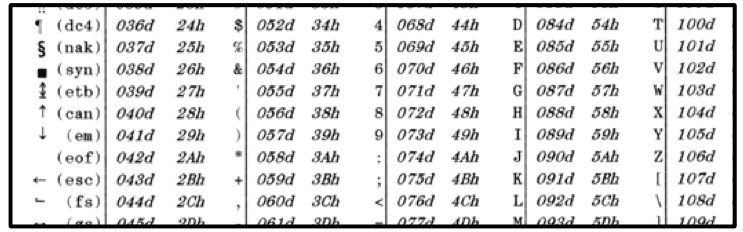
\includegraphics[width=0.7\textwidth]{images/ascii.png}
\end{center}

\end{frame}

\begin{frame}{Example 16 (1/2)}

\lstinputlisting[firstline=214,lastline=223,language=c]{../../code/mrk-board/intro_examples/sources/main.c}

\end{frame}

\begin{frame}{Example 16 (2/2)}

\lstinputlisting[firstline=224,lastline=231,language=c]{../../code/mrk-board/intro_examples/sources/main.c}

\end{frame}

\begin{frame}{Lessons}

\begin{enumerate}
\def\labelenumi{\arabic{enumi}.}
\tightlist
\item
  Table

  \begin{itemize}
  \tightlist
  \item
    declaration and use
  \end{itemize}
\end{enumerate}

\end{frame}

\begin{frame}{Example 17 (1/3)}

\lstinputlisting[firstline=233,lastline=243,language=c]{../../code/mrk-board/intro_examples/sources/main.c}

\end{frame}

\begin{frame}{Example 17 (2/3)}

\lstinputlisting[firstline=244,lastline=258,language=c]{../../code/mrk-board/intro_examples/sources/main.c}

\end{frame}

\begin{frame}{Example 17 (3/3)}

\lstinputlisting[firstline=260,lastline=275,language=c]{../../code/mrk-board/intro_examples/sources/main.c}

\end{frame}

\begin{frame}{Lessons}

\begin{itemize}
\tightlist
\item
  A calculator
\item
  Type casting
\end{itemize}

\end{frame}


%====================
%=== bibliography ===
%====================

\end{document}